\documentclass[10pt]{article}
\usepackage{cite}
\usepackage{fancyhdr}
\usepackage[svgnames]{xcolor}
\usepackage{url}
\usepackage{tikz}
\usetikzlibrary{shapes,snakes,arrows}
\usepackage{hyperref}
\usepackage{graphicx}
\usepackage[complexity, primitives]{cryptocode}

\topmargin=-5mm
\evensidemargin=0cm
\oddsidemargin=0cm
\textwidth=16cm
\textheight=22cm
\addtolength{\headheight}{1.6pt}
\hypersetup{pdfstartview=}

\tikzset{>=latex}

\newcommand{\secref}[1]{\S\ref{#1}}

\newcommand{\lastupdate}{\today}
\newcommand{\ie}{\textit{i.e.}}
\newcommand{\mdash}{---}
\newcommand{\ecall}{\textsf{ecall}}
\newcommand{\ocall}{\textsf{ocall}}
\newcommand{\env}{\textsf{environment}}
\newcommand{\mrenclave}{\textsf{mrenclave}}
\newcommand{\mrsigner}{\textsf{mrsigner}}
\newcommand{\sha}{\textsf{sha256}}
\newcommand{\pve}{\textsf{PvE}}
\newcommand{\pce}{\textsf{PcE}}
\newcommand{\qe}{\textsf{QE}}
\newcommand{\launchenclave}{\textsf{Launch Enclave}}
\newcommand{\uc}{\textsf{UC}}

% \lhead{\sc On the insufficiency of Intel SGX Remote Attestation}
% \rhead{\sc \lastupdate}

\title{\bf A Framework for analyzing Intel SGX Enclaves}
\author{\textsc{Yogesh Prem Swami}}

\date{\lastupdate}

\begin{document}
\pagenumbering{arabic}

\maketitle

\begin{abstract}
  Intel SGX enclaves  provide hardware
  enforced confidentiality and integrity guarantees for running pure
  computations (\ie, OS-level side-effect-free code) in the cloud
  environment. In addition, SGX remote attestation enables
  enclaves to prove that a claimed enclave is indeed running inside a
  genuine SGX hardware and not some (adversary controlled) SGX
  simulator.

  Since cryptographic protocols do not compose well \cite{ucframework}, 
  especially when run concurrently, SGX remote attestation is only a 
  necessary pre-condition for securely instantiating an enclave. In 
  practice, one needs to analyze all the different interacting enclaves 
  as a single protocol and make sure that no sub-computation of the 
  protocol can be simulated outside of the enclave. In this paper, 
  we present a practical framework for analyzing enclaves. We analyze 
  Intel provided EPID\cite{epid} \textsf{Provisioning} and \textsf{Quoting} 
  Enclave\cite{sgxattest} within this framework and report our (largely 
  positive) findings. We also provide details about SGX's use of EPID 
  and report (largely negative) results about claimed anonymity guarantees.
  
\end{abstract}

\section{Introduction}
\label{sec:intro}
  Intel SGX enclaves\cite{sgxinnov, sgxinnov2} provide hardware
  enforced confidentiality and  integrity guarantees for running pure
  computation (\textit{i.e.}, OS-level side-effect-free code) in the
  cloud environment. By limiting the application's Trusted Computing
  Base (TCB) to the CPU and CPU-Cache, SGX provides unprecidented
  confidentiality and integrity guarantees against malicious OS
  kernels and supervisor software. A popular design methodology---as 
  evidenced by \cite{Haven, Graphene, Scone}---for creating secure 
  cloud applications is as follows:

  \begin{description}
    \item[Step-1:] Define a remote-attestation mechanism to securely 
      instantiate an enclave. Quite often, this step is not explicitly 
      stated probably because a generic black-box attestation 
      scheme---whatever that means---is expected to suffice.
    \item[Step-2:] Then, largely independently of the remote-attestation 
      mechanism, define the functionlity that needs to be implemented 
      inside the enclave. This step often involves composing different 
      cryptographic as well as non-cryptographic protocols as the 
      application algorithm demands.
    \item[Step-3:] Finally, define a ``run-time workflow," where one first
      validates the remote-attestation result, and then runs the algorithm
      implemented in the enclave.
  \end{description}

  This approach, while modular and elegant from software engineering
  perspective, is not always secure. As pointed out in 
  \cite{ucframework}, unless a protocol is desgined for 
  ``\textsf{Universal Composition}" (\uc)---where, the real-world 
  behavior and the ideal-world definition (function) of a protocol 
  are computationally indistinguishable \textit{for every} adversary 
  controlled environment---it's unlikely that arbitrary composition 
  of protocols will be secure. On the other hand, proving results in 
  the \uc-framework is rather difficult and sometimes it's unclear 
  whether the proof doesn't work because of technical difficulties 
  or whether the protocol itself is insecure.

  We illustrate the problem associated with the protocol composition 
  with two real-world examples. To set the stage, a cloud service 
  provider\footnote{This example is based on an actual protocol 
  designed by a mid-sized cloud-security/compliance firm.} wanted to 
  migrate its new clients from Amazon Cloud-HSM to an SGX enclave. 
  The protocol for interacting with the enclave was based on 
  HTTP Request/Response framework, where different operations (such as
  \textsf{KeyGen}), were sent as a command, and the enclave would execute
  them using a single function call.

  Important use-case for the enclave was to support (a) local key 
  generation, (b) storing the private-key on disk encrypted with a 
  scheme that would allow fast key-lookup, (c) creating Certificate 
  Sining Requests (CSR) using challenge-response protocol 
  \cite[\S5.2.8.3]{rfc4210}, and (d) installing AEAD encrypted 
  certificate with the corresponding private key on disk as a single
  key entity.

  \subsection{Sequential Protocol Composition}

  In this paper, we present a way to analyze Intel SGX enclaves, which is
  a compromize between ad-hoc protocol composition and full \uc-based 
  analysis. The analysis framework exploits the SGX computational model, and 
  describes a few possible ways of attacking an SGX enclave.

  \section{SGX Computational Model}
  \label{sec:model}
  Intel documentation\cite{intelsdm} provides excellent low-level
  details about the SGX instructions. This section provides an
  abstract computational model of SGX which is better suited for
  security analysis of an SGX enclave.

  Abstractly, an SGX enclave can be thought of as a blackbox that's
  capable of running any arbitrary algorthim. The blackbox, hereafter
  called an enclave, communicates with the outside world, called the
  \env, in three different ways:

  \begin{figure}[h]
  \centering
  \label{fig:model}
  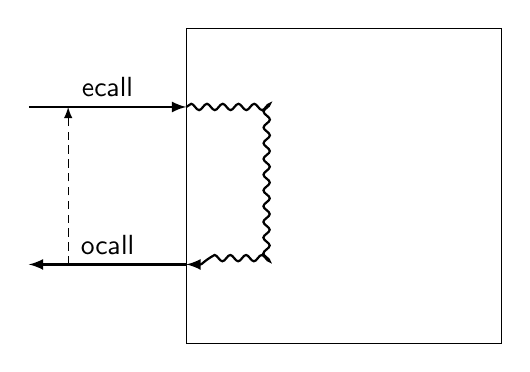
\begin{tikzpicture}[x=1cm, y=-1cm]
  \newcommand{\ench}{4cm}
  \newcommand{\encw}{4cm}
  \newcommand{\alen}{1cm}
  \newcommand{\adiff}{1cm}

  \node[rectangle, minimum height=\ench, minimum width=\encw, draw] (enc) {};
  \draw[->,thick] (-\encw / 2.0 - 2*\alen, \adiff ) -- (-\encw/2.0, \adiff) %%
  node [midway, above] {\textsf{ecall}};

  \draw [->, thick, decorate, %%
    decoration={snake,amplitude=.4mm,segment length=2mm, post length=1mm}] %%
  (-\encw/2.0, \adiff) -- (-\encw/2.0 + 1*\adiff + 0.1, \adiff) -- %%
  (-\encw/2.0 + 1*\adiff , -\adiff) -- (-\encw/2.0, -\adiff);


  \draw[<-,thick] (-\encw / 2.0 - 2*\alen, -\adiff ) -- (-\encw/2.0, -\adiff) %%
  node [midway, above] {\textsf{ocall}};

  \draw[->, thin,densely dashed] (-\encw / 2.0 - 1.5*\alen, -\adiff ) -- %%
  (-\encw/2.0 - 1.5*\alen , \adiff);
\end{tikzpicture}

  \caption{SGX Computational Model.}
  \end{figure}

  \begin{description}
  \item[Ecall]: The \env\ can invoke a pre-defined function inside the
    enclave by passing input parameters and returning internal state
    of the enclave as results. Such invocations from the \env\ to the
    enclave are referred to as \ecall. The parameter values passed
    from the \env\ to the enclave are either copied or directly shared
    with the enclave. An \ecall\ can terminate in one of the three
    ways: (a) by returning from the enclave, (b) by making an explicit
    \ocall, or (c) as a result of an interrupt or exception.

    SGX also supports multithreading, and it's possible for the
    \env\ to run the same \ecall\ in different threads. However, once
    an \ecall\ has acquired the thread, future attempts to reuse that
    same thread will result in error. Futhermore, the number of
    threads that an enclave can support is pre-determined by the
    enclave signer, and cannot be altered at runtime.

  \item [Ocall]: While an enclave is executing (because of some
    previous \ecall), it can make \ocall s  to pre-designated
    functions in the \env.  Unlike an \ecall, an \ocall\ cannot
    directly share the internal enclave state with the \env, and
    must---directly or indirectly---copy the parameters into the
    \env\ before making an \ocall.

    An interesting characteristic of an \ocall\ is that the \env\ is
    not requred to return back to the enclave at the end of the
    \ocall\ (see Figure~\ref{fig:model}). Since the behavior of pre-designated
    functions in the \env\ are controlled by the adversary, one should
    not expect the \env\ to follow the protocol that enclave author
    envisioned. In particular, it's possible to create a chain of
    \ecall s and \ocall s such that the adversary can perform
    operations on the internal (global) state of the enclave.

  \item[Asynchrnonous Exit]: In addition to an \ocall, the
    processor can exit from an enclave due to an interrupt or
    exception. Such enclave exiting events are called Asynchronous
    Exit Events, or AEX. Unlike an \ocall, an AEX can transfer control
    from the enlave to the environment at arbitrary (possibly adversary
    controlled) points inside the enclave. Like \ocall s, an AEX can
    either by resumed from where the enclave left off, or the
    environment can invoke another \ecall (either within the same
    thread or a different thread).

    Since an adversary can create multiple running copies of an
    enclave and selectively interrupt each enclave to cause and AEX,
    it can be used as a means to ``rewind'' the internal state of of
    the enclave. Given that proof-of-knowledge \cite{BellarePOK}
    protocols fundamentally have a \textit{knowledge-extractor} based
    on rewinding, an enclave must ensure that it does not leak secrets
    when interrupted by an AEX.

  \end{description}

  \subsection{Enclave Creation}
  \label{sec:enclavecreateion}
  An enclave is generated as a dynamically shared library using
  standard compiler tools. In addition, the entity creating the
  enclave must also decide up-front on the following information:

  \begin{description}
    \item[Attributes]: The attributes of an enclave act as an access
      control mechanism that is enforced by the hardware. For example,
      certain high priviledge keys, such as Launch-Key and Provision-Key
      cannot be made accessible to all the enclaves, as it would
      compromize the security of entire SGX ecosystem---not just a
      given CPU. An enclave author requests the attributes needed by
      the enclave at compiler/sign time, and the Launch-Enclave, based
      on policy decisions, decides whether to grant or reject an
      authorization token (called \textsf{EINITTOKEN}) for instantiating
      the enclave.
    \item[Stack size]: The enclave author must estimate the size of the
      stack needed by enclave and set its value at enclave creation time.
      Once an enclave is instantiated, this value cannot be changed.

    \item[Heap size]: Like the stack size, the heap-size of the enclave
      is also fixed at enclave creation time. In SGXv2, this value can
      be changed post instantiation.

    \item[Thread count]: An enclave must also decide upon the number
      of threads that can run conconrrently. As pointed out in
      \secref{sec:model}, concurrency can have a dramatically negative
      impact on the security of the certain protocols, and one must
      not select this parameter just on the basis of performance
      requirements, but also on the basis of security concerns.

    \item[Software versioning]: SGX provides elaborate software-upgrade
      and life-cycle management faciliaties and allows software vendors
      to make use of these features.

  \end{description}
  Based on these parameters, the enclave signing tool creates a
  virtual memory layout of the enclave and comptes a hash of the
  entire memory layout (including the stack, heap, thread control
  structure, etc.)  See \cite{intelsdm} for details
  about how the hash is computed. This hash, called
  \mrenclave, is used as the unique identifier for the enclave.

  In addition to \textsf{mrenclave}, the software vendor must
  also sign the enclave using a RSA-3072 key. The hash of the RSA
  Public-Key is called \mrsigner. As described in \cite{surnaming},
  the purpose of the signature is to provide an unforgeable
  identity---a \textit{surname} based lineage---to a set of enclaves
  based on the vendor.

  It should be noted that the \mrenclave\ of an enclave doesn't
  change even when the signing key is changed. This is significant
  when validating attestation or deriving keys based on
  \mrenclave.

  \subsection{Enclave Instantiation and Access Control}
  A properly signed enclave can be instantiated on any Intel
  SGX Processor---subject to access control restrictions enforced
  by \launchenclave. Before an enclave can be instantiated on an SGX capable
  processor, it must get an authorization token,
  called \textit{Launch Token}, from Intel provided \launchenclave. The
  \launchenclave\ uses a combination of \mrenclave, \mrsigner, the
  attributes of the enclave and a \textit{whitelist signed by Intel} to decide
  whether to grant Launch Token to the enclave or not. Once an
  enclave obtains a Launch Token, the enclave  can continue
  using it indefinitely, even when the policies of the \launchenclave\
  might get updated later on.

  \subsection{SGX Platform Keys}
  As described in \cite{sgxattest}, each Intel SGX capable processor
  contains two statistically independent base keys:
  \textit{Root Provisioning Key} and \textit{Root Seal Key}. The Root
  Provisioning Key is used as the Root of trust between the CPU and
  Intel Attestation Services (IAS) \cite{ias}. Intel retains a copy
  of this key at the time of manufacturing and uses it to establish
  the trustworthiness of the processor during EPID join process. Intel
  claims that Root Seal Key is not retained. However, it's not clear
  whether the this key is generated inside the processor via oracle
  access (\ie, in such a way that CPU generates the key all by itself
  using it's own internal random numbers or with PUFs), or whether the
  key is first generated outside the processor, then injected into CPU,
  and finally all outside references destroyed. Unless these keys are
  generated via oracle access, one should consider the Root Seal Key
  to be known to Intel.

  \begin{figure}[h]
  \centering
  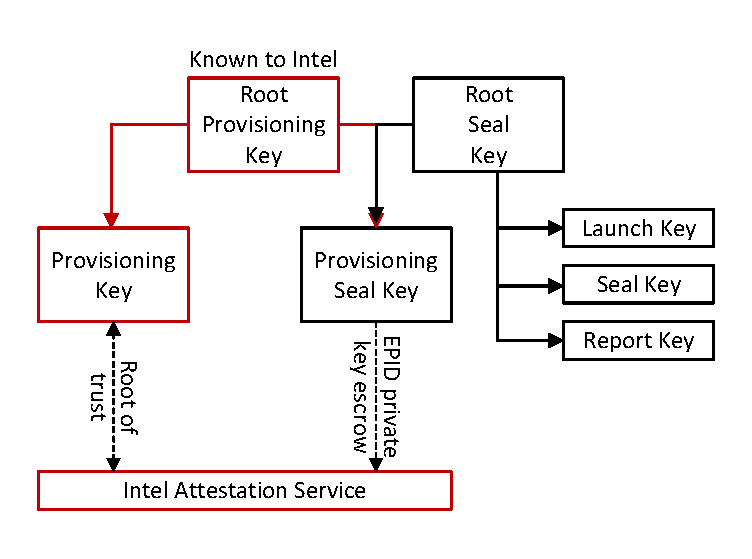
\includegraphics[scale=.75]{Diagrams/KeyHierarchy}
  \caption{Intel SGX Platform Keys}
  \label{fig:keys}
  \end{figure}

  An application software does not have raw acceess to these base
  keys. However, an application can access following \textit{named}
  keys that are derived from these two base key (see
  Figure~\ref{fig:keys}):

  \begin{description}
    \item[Provisioning Key]: This key is derived from
      Provisioning Key and is used as the root-of-trust
      between the CPU and the Intel Attestation Service during the
      EPID join process. Since admitting a non-SGX processor to
      the Intel Attesttion Service's group of SGX Processors will
      completely compromize Remote Attestation of all CPUs, extreme
      care must be taken in granting access to Provisioning Key.
      Currently, the \launchenclave\ only grants Provisioning Key
      access to enclaves that have been signed by Intel. Furthermore,
      only Provisioning Enclave (\pve) and Provisioning Certification
      Enclave (\pce) (both created without debug option) have access to
      Provisioning Key.

    \item[Provisioning Seal Key]: This key is derived joinly from Root
      Provisioning Key and Root Seal Key. The EPID join process, the
      EPID private-key for each platform is encrypted with this key
      and uploaded to Intel Attestation Service. (See \secref{ssec:epidprov}
      for details about EPID join process.)

      Note that the EPID private-key could not just be encrypted with
      Provisioning Key as that would destory the EPID's blinded-join
      protocol. Conversely, the EPID private-key cannot be encrypted
      just with Seal Key as that might allow non-priviledged enclaves
      to have access to EPID private key and thereby render Remote
      Attestation ineffective\footnote{If someone could access EPID
      private key---either directly, or through oracle access---they
      could sign remote attestation queries for \textit{any}
      platform. Furthermore, because of anonymimity, it will be
      impossible to determine which platform was abused in this way.}.

      In spite of this design choice, given the uncertainity about
      how the Root Seal Key is generated, one should assume that
      Intel knows the EPID private key for each platform.

      \item[Launch Key]: This key is derived from Root Seal Key and
      is used by \launchenclave\ to create authorization tokens
      (\textsf{EINITTOKEN}) that each non-Intel enclave must obtain
      in order to instantiate an enclave. Only a specific
      \mrsigner---whose corresponding private-keys are only known
      to Intel---can access the Launch Key. In SGXv2, the \mrsigner\
      for \launchenclave\ can be changed programatically,
      (see \cite[\S39.1.4]{intelsdm} for details) and any enclave
      signed with that \mrsigner\ can gain access. With
      this change, however, it's not clear how Intel intends
      to enforce access control restrictions on the
      Proviosioning Key.

      \item[Seal Key]: This key is derived from Root Seal Key and used
      for encrypting data specifically for a given CPU.

      \item[Report Key]: This key is derived from Root Seal Key and used
      for Local Attestation (see \secref{sec:localatt} for detailed
      information on Local Attestation how Report Key is used).

  \end{description}

  In addition to the named keys, each key can be further diversified using
  a 128-bit user selected constant called \textit{Key Wearout Protection}. 
  In addition, certain keys can be further diversified using \mrenclave\ 
  or \mrsigner\ of the enclave.

  \section{Framework for Analyzing SGX Enclave}
  \label{sec:analysisfwk}

  While an SGX enclave is generally presented as a programming tool
  to conceal the computational state of an algorithm, in practice each
  enclave implements a protocol between the \env\ and the algorithm that
  the enclave implements. The \ocall s, \ecall s, and AEX define the 
  external interface for interacting with the protocol. An enclave can be
  considered secure only if the \textit{overall protocol} implemented 
  by the enclave is secure.

  As described in \secref{sec:intro}, sequential, concurrent, and parallel
  composition of otherwise secure protocols, does not necessarily result
  in an overall secure system. One way to formalize the overall security
  of an enclave would be consider the 

  \subsection{Concurrent Enclave Execution}
  \label{ssec:concexec}

  \subsection{Parallel Enclave Execution}
  \label{ssec:parallelexec}

  \subsection{Enclave Rewinding}
  \label{ssec:rewinding}

  \section{Local Attestation}
  \label{sec:localatt}

  \section{SGX Remote Attestation}
  \label{sec:remoteatt}

  \subsection{EPID Overview}
  \label{ssec:epid}

  \subsection{SGX Pairing Groups}
  \label{ssec:pairings}

  \subsection{SGX EPID provisioning}
  \label{ssec:epidprov}

  \subsection{SGX Quoting Enclave}
  \label{ssec:qe}

  \section{Conclusion}
  \label{sec:conclusion}

\bibliographystyle{alpha}
\bibliography{sgx_biblio}

\end{document}